\section{Results}
\label{sec:results}
\subsection{Prediction on excluded cohorts and reference baselines}
\label{sec:results_prediction}
Under the controlled $L_2$ logistic classifier, four-cohort mean AUROC across the five primary selectors ranged from 0.628 (Stability Selection, $\pi \ge 0.60$) to 0.731 (Elastic Net), with LASSO at 0.728 and TENTACLES at 0.723; mean balanced accuracy ranged from 0.563 to 0.655, highest for TENTACLES, which also achieved the highest mean AUPRC (0.843), F1 (0.704) and lowest Brier score (0.236) (Table~\ref{tab:results_main}; complete per-cohort eight-metric table with 2,000-resample 95\% bootstrap CIs in Table~\ref{tab:s1}). Method-native predictors differed notably in some cases (for example, native StableMate achieved mean AUROC 0.743 and balanced accuracy 0.624 versus 0.659 and 0.598 under the controlled classifier), illustrating why separating feature selection from downstream classification clarifies method comparisons.

\begin{table*}[!t]
\caption{Controlled five-method benchmark and reference baselines under identical class-balanced $L_2$ logistic regression ($C=1$; CD positive). AUROC and BA (balanced accuracy) are unweighted four-cohort means with sample SD ($n-1$ denominator). LOCO mean pairwise Jaccard ($\bar{J}$) averages six dependent fold pairs; Monte Carlo (MC) nulls are size-only chance references (10,000 draws), not dependence-calibrated hypothesis tests.}
\label{tab:results_main}
\centering\scriptsize
\resizebox{\textwidth}{!}{\begin{tabular}{@{}llrrrrrrrl@{}}
\toprule
Selector / Baseline & Role & Panel mean [min--max] & AUROC (SD) & BA (SD) & AUPRC & F1 & Brier & LOCO $\bar{J}$ (Obs / MC Null) & All 4\\
\midrule
Elastic Net & Primary & 124.3 [11--430] & 0.731 (0.103) & 0.583 (0.063) & 0.812 & 0.633 & 0.313 & 0.092 / 0.002 (49.1$\times$) & 0\\
LASSO & Primary & 120.0 [77--219] & 0.728 (0.067) & 0.620 (0.023) & 0.825 & 0.697 & 0.310 & 0.102 / 0.006 (16.2$\times$) & 2\\
TENTACLES & Primary & 76.5 [61--91] & 0.723 (0.100) & \textbf{0.655} (0.093) & \textbf{0.843} & \textbf{0.704} & \textbf{0.236} & \textbf{0.210} / 0.005 (46.3$\times$) & 6\\
StableMate & Primary & 15.8 [14--20] & 0.659 (0.083) & 0.598 (0.110) & 0.801 & 0.642 & 0.310 & 0.033 / 0.001 (34.9$\times$) & 0\\
Stability Selection\ ($\pi\ge 0.60$) & Primary & 6.3 [4--9] & 0.628 (0.051) & 0.563 (0.050) & 0.797 & 0.656 & 0.258 & 0.128 / 0.0004 (338.2$\times$) & 0\\
\midrule
All-9,983 Shared Genes & Baseline & 9,983 (all) & 0.681 (0.073) & 0.572 (0.035) & 0.775 & 0.659 & 0.336 & --- & ---\\
Train-Eligible ($\ge 10\%$) & Baseline & 8,397.5 [8,337--8,438] & 0.673 (0.130) & 0.592 (0.076) & 0.764 & 0.624 & 0.371 & --- & ---\\
\texttt{limma-voom} Top-10 & Baseline & 10 (fixed) & 0.748 (0.101) & 0.631 (0.094) & 0.856 & 0.723 & 0.215 & --- & ---\\
\texttt{limma-voom} Top-100 & Baseline & 100 (fixed) & 0.710 (0.117) & 0.649 (0.106) & 0.814 & 0.705 & 0.236 & --- & ---\\
Welch $t$-test Top-10 & Baseline & 10 (fixed) & 0.772 (0.081) & 0.601 (0.081) & 0.867 & 0.625 & 0.254 & --- & ---\\
Welch $t$-test Top-100 & Baseline & 100 (fixed) & 0.732 (0.083) & 0.660 (0.064) & 0.842 & 0.722 & 0.228 & --- & ---\\
\bottomrule
\end{tabular}}
\end{table*}

\begin{figure*}[!t]
\centering
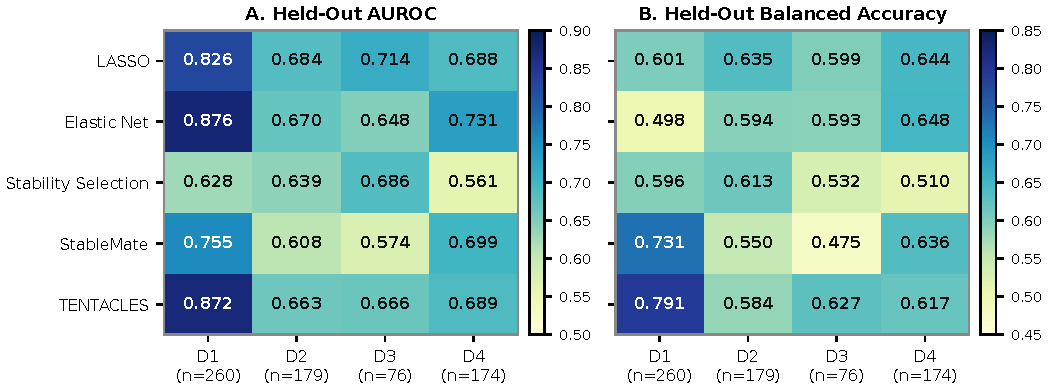
\includegraphics[width=\textwidth]{heldout_metric_heatmaps.pdf}
\caption{External test performance of all five feature-selection methods, separately for each left-out cohort under the identical fixed class-balanced $L_2$ logistic classifier ($C=1$). Entries show (A) AUROC and (B) balanced accuracy at probability threshold 0.5. Cohort sample counts are given below D1--D4; darker cells indicate higher values.}
\label{fig:results_heatmap}
\end{figure*}

Performance depended strongly on the held-out cohort, and within-cohort 95\% bootstrap CIs overlapped substantially across methods (Fig.~\ref{fig:results_heatmap} and Fig.~\ref{fig:tradeoff}B). On D1, Elastic Net (0.876 [0.831, 0.918]) and TENTACLES (0.872 [0.819, 0.916]) attained the highest AUROCs, whereas Stability Selection obtained 0.628 [0.531, 0.717]. On D2 and D3, LASSO led (0.684 and 0.714); on D4, Elastic Net led (0.731). While D1 and D4 occupy positive PC1 coordinates in Fig.~\ref{fig:pca}, this visual proximity is strictly an exploratory observation rather than a causal explanation for D1 performance, as D1 also has the highest CD prevalence (83.8\%) and uniform ileal biopsies.

Reference baselines under the identical classifier provided an essential anchor (Table~\ref{tab:results_main}; Tables~\ref{tab:s2}--\ref{tab:s3}). All-9,983 shared genes achieved mean AUROC 0.681 (SD 0.073; BA 0.572) and Train-Eligible ($\ge 10\%$) achieved 0.673 (sample SD 0.130; BA 0.592). Training-only univariate differential expression achieved competitive discrimination across the entire $K\in\{10,25,50,100,200\}$ curve (\texttt{limma-voom}: 0.748 at $K=10$ to 0.710 at $K=100$; Welch: 0.772 at $K=10$ to 0.732 at $K=100$; reported descriptively without post-hoc selection of a single best $K$). Size-matched random panels ($B=100$) attained strong baseline AUROCs on D1 (mean 0.794--0.796 for $K=73$--$94$) and D4 (0.681--0.685), with only a minority of the 20 method-cohort cells falling below descriptive $p_{\mathrm{emp}} < 0.05$ (for example, Elastic Net on D1 at $K=11$, $p_{\mathrm{emp}}=0.0099$; TENTACLES on D1 BA, $p_{\mathrm{emp}}=0.0396$).

\subsection{TENTACLES consensus-vote sensitivity}
\label{sec:results_tentacles}
The TENTACLES six-of-nine consensus produced panels of 73, 91, 81 and 61 genes (D1--D4). The primary rule gave mean AUROC 0.723 and mean balanced accuracy 0.655. Relaxing the consensus to five votes selected 90--115 genes per fold and reduced mean AUROC to 0.691 (Table~\ref{tab:tentacles_sensitivity}). Six votes scored higher on D1, D3 and D4, but not on D2; it should not be described as uniformly superior.

\begin{table}[!t]
\caption{TENTACLES on each held-out cohort: prespecified 6/9-vote primary versus 5/9-vote sensitivity. AUROC intervals are 95\% patient-stratified bootstrap intervals (2,000 resamples), conditional on the fitted six-vote model.}
\label{tab:tentacles_sensitivity}
\centering\footnotesize
\setlength{\tabcolsep}{2.9pt}
\renewcommand{\arraystretch}{1.1}
\begin{tabular}{@{}lcccc@{}}
\toprule
Test & 6-vote genes & 6-vote AUROC [95\% CI] & 6-vote BA & 5-vote AUROC\\
\midrule
D1 & 73 & 0.872 [0.819, 0.916] & 0.791 & 0.824\\
D2 & 91 & 0.663 [0.565, 0.756] & 0.584 & 0.666\\
D3 & 81 & 0.666 [0.529, 0.796] & 0.627 & 0.647\\
D4 & 61 & 0.689 [0.604, 0.760] & 0.617 & 0.626\\
\midrule
Mean & 76.5 & 0.723 & 0.655 & 0.691\\
\bottomrule
\end{tabular}
\end{table}

\subsection{Gene-panel agreement and fixed-$K$ sensitivity}
\label{sec:results_genes}
The relationship between predictive transfer and gene-set agreement was not monotonic (Fig.~\ref{fig:tradeoff}A; Fig.~\ref{fig:overlap}A; Table~\ref{tab:s4}). Under LOCO, TENTACLES achieved the highest observed mean pairwise Jaccard (0.210 vs.\ 0.005 size-only MC null, $46.3\times$; overlap coefficient 0.383) and six genes present in all four panels (\textit{CLDN18}, \textit{FFAR2}, \textit{MMP3}, \textit{NOS2}, \textit{PAQR5} and \textit{PML}; exact four-way size-only expectation $5.44\times 10^{-5}$). Stability Selection achieved 0.128 vs.\ 0.0004 ($338.2\times$, driven by 4--9 gene panels; zero four-way genes), LASSO achieved 0.102 vs.\ 0.006 ($16.2\times$; two four-way genes: \textit{CLIC6}, \textit{ZNF727}), Elastic Net achieved 0.092 vs.\ 0.002 ($49.1\times$; zero four-way) and StableMate achieved 0.033 vs.\ 0.001 ($34.9\times$; zero four-way).

\begin{figure*}[!t]
\centering
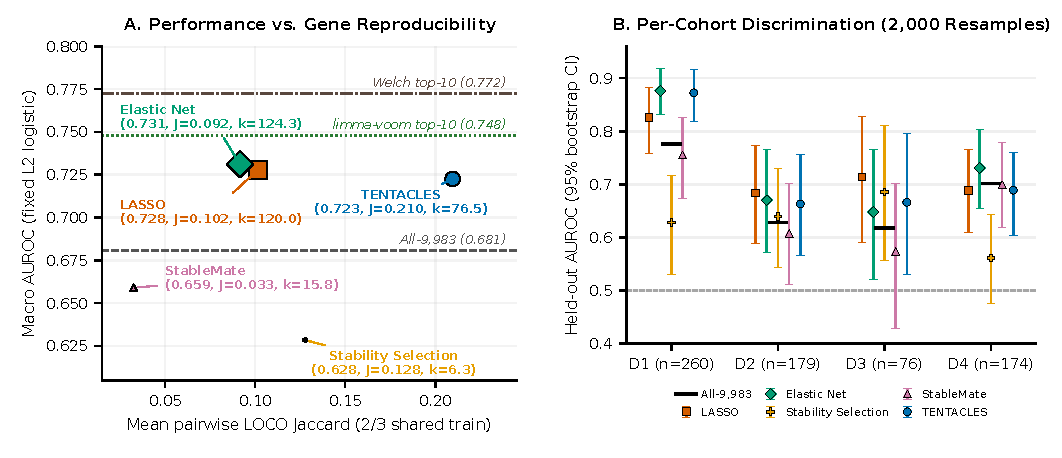
\includegraphics[width=\textwidth]{prediction_vs_agreement.pdf}
\caption{Prediction--reproducibility trade-off and per-cohort uncertainty. (A) Four-cohort mean held-out AUROC versus mean LOCO gene Jaccard (bubble area proportional to mean panel size $k$), anchored against All-9,983, \texttt{limma-voom} top-10 and Welch top-10 baselines. (B) Per-cohort AUROC with 2,000-resample stratified bootstrap 95\% CIs across D1--D4.}
\label{fig:tradeoff}
\end{figure*}

\begin{figure*}[!t]
\centering
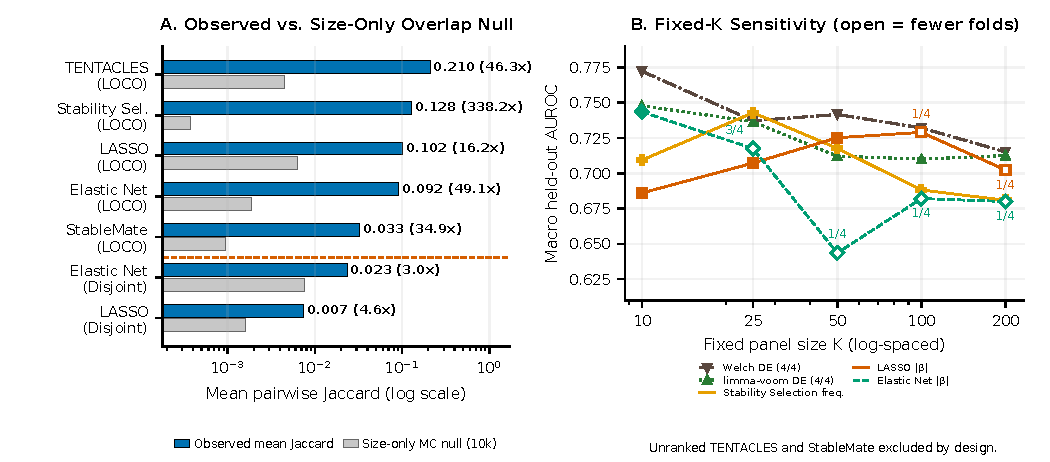
\includegraphics[width=\textwidth]{overlap_null_and_fixedK.pdf}
\caption{(A) Observed mean pairwise Jaccard versus size-only 10,000-draw Monte Carlo null across LOCO and disjoint single-cohort fits. (B) Fixed-$K$ sensitivity across continuously ranked methods; solid markers denote 4/4 evaluable folds, whereas open markers denote partial support ($<4/4$ folds) and must not be equated to four-fold means.}
\label{fig:overlap}
\end{figure*}

In patient-disjoint single-cohort fits, LASSO selected 27, 92, 9 and 31 genes for D1--D4, respectively, while Elastic Net selected 152, 198, 109 and 91 genes (Table~\ref{tab:independent_sizes}). All LASSO single-cohort fits selected fewer genes than the number of samples in the corresponding cohort. Across these disjoint cohorts, mean pairwise Jaccard was 0.007 for LASSO and 0.023 for Elastic Net, with no genes shared across all four independent fits.

\begin{table}[!t]
\caption{Gene panel sizes selected in disjoint single-cohort fits. These panels were not used for held-out prediction.}
\label{tab:independent_sizes}
\centering\scriptsize
\setlength{\tabcolsep}{2.4pt}
\resizebox{\columnwidth}{!}{\begin{tabular}{@{}lrrrrrl@{}}
\toprule
Selector / Solver & D1 & D2 & D3 & D4 & $\bar{J}$ (Obs/Null) & 4-Way\\
\midrule
LASSO (\texttt{liblinear}) & 27 & 92 & 9 & 31 & 0.007 / 0.002 & 0\\
Elastic Net (\texttt{glmnet}) & 152 & 198 & 109 & 91 & 0.023 / 0.008 & 0\\
\bottomrule
\end{tabular}}
\end{table}

\begin{table}[!t]
\caption{Fixed-$K$ panel-size sensitivity for continuously ranked methods. Partial-support means ($<4/4$ folds) are flagged explicitly and are not comparable to four-fold means.}
\label{tab:fixedk}
\centering\scriptsize
\setlength{\tabcolsep}{3.2pt}
\resizebox{\columnwidth}{!}{\begin{tabular}{@{}lrrlrr@{}}
\toprule
Method & $K$ & Folds & Cohorts & AUROC & BA\\
\midrule
LASSO & 10 / 25 / 50 & 4/4 & D1--D4 & 0.686 / 0.707 / 0.725 & 0.613 / 0.626 / 0.628\\
LASSO & 100 / 200 & 1/4 & D3 only & 0.729 / 0.702 & 0.605 / 0.587\\
Elastic Net & 10 & 4/4 & D1--D4 & 0.744 & 0.596\\
Elastic Net & 25 & 3/4 & D2--D4 & 0.717 & 0.620\\
Elastic Net & 50 / 100 / 200 & 1/4 & D3 only & 0.644 / 0.682 / 0.680 & 0.529 / 0.573 / 0.608\\
Stability Selection\ (rank) & 10 / 25 / 50 & 4/4 & D1--D4 & 0.709 / 0.743 / 0.718 & 0.613 / 0.598 / 0.588\\
Stability Selection\ (rank) & 100 / 200 & 4/4 & D1--D4 & 0.688 / 0.681 & 0.608 / 0.575\\
TENTACLES & 10--200 & 0/4 & None & \multicolumn{2}{c}{Unranked consensus (excluded)}\\
StableMate & 10--200 & 0/4 & None & \multicolumn{2}{c}{Unranked consensus (excluded)}\\
\bottomrule
\end{tabular}}
\end{table}

In fixed-$K$ sensitivity (Table~\ref{tab:fixedk}; Fig.~\ref{fig:overlap}B), Stability Selection (ranked frequency, evaluable on 4/4 folds across all $K$) rose from mean AUROC 0.628 ($\pi \ge 0.60$, mean 6.3 genes) to 0.709 at $K=10$ and 0.743 at $K=25$ before tapering to 0.681 at $K=200$. This shows that Stability Selection performance is sensitive to the number of ranked genes and is consistent with a small-panel handicap, although varying $K$ simultaneously alters gene membership, ranking truncation and downstream regularisation fit rather than isolating a single causal mechanism. LASSO was evaluable on 4/4 folds through $K=50$ and only 1/4 folds (D3, $n_{\mathrm{nonzero}}=219$) at $K=100,200$; Elastic Net was evaluable on 4/4 folds at $K=10$, 3/4 at $K=25$, and 1/4 (D3, $n_{\mathrm{nonzero}}=430$) at $K\ge 50$.

\subsection{Reactome pathway overlap and D3 QC sensitivity}
\label{sec:results_pathways}
Table~\ref{tab:results_pathways} summarises Reactome v98 enrichment for the TENTACLES, Stability Selection and StableMate panels. TENTACLES yielded 0, 11, 8 and 9 significant pathways across D1--D4, respectively (mean pathway Jaccard 0.256), including recurring interleukin-signalling and G-protein-coupled receptor pathways in D2--D4. Stability Selection and StableMate yielded no significant pathways in the assessed folds. Enrichment was not recalculated for the final LASSO or Elastic Net panels; their pathway results are therefore not reported or interpreted here.

\begin{table}[!t]
\caption{Reactome v98 enrichment ($q<0.05$) for gene panels with available final-analysis pathway results. A dash indicates that pathway agreement cannot be calculated when no significant pathways are present.}
\label{tab:results_pathways}
\centering\footnotesize
\setlength{\tabcolsep}{3.5pt}
\begin{tabular}{@{}lccc@{}}
\toprule
Method & D1/D2/D3/D4 & Folds & $\bar{J}$\\
\midrule
TENTACLES & 0/11/8/9 & 3/4 & 0.256\\
Stability Selection & 0/0/0/0 & 0/4 & ---\\
StableMate & 0/0/0/0 & 0/4 & ---\\
\bottomrule
\end{tabular}
\end{table}

Finally, excluding the seven source-flagged \texttt{qc=EXCLUDE} D3 samples in held-out test-only rescoring ($n=69$; Table~\ref{tab:s5}, Fig.~\ref{fig:s1}B) yielded small AUROC shifts for LASSO ($-0.005$), Elastic Net ($+0.002$), Stability Selection ($-0.015$) and StableMate ($-0.020$), and an increase of $+0.061$ for TENTACLES (AUROC $0.666 \to 0.726$; BA $+0.035$). Because D1, D2 and D4 were not retrained without these seven rows, these shifts quantify held-out test sensitivity rather than full-retraining sensitivity.
